\documentclass[12pt]{article}
%Some packages I commonly use.
\usepackage[english]{babel}
\usepackage{graphicx}
\usepackage{framed}
%
\usepackage{scrextend}
\usepackage{tocloft}
\usepackage{multirow}
\usepackage{xcolor}
%
\usepackage[normalem]{ulem}
\usepackage{amsmath}
\usepackage{amsthm}
\usepackage{amssymb}
\usepackage{amsfonts}
\usepackage{enumerate}
\usepackage[utf8]{inputenc}
\usepackage[utf8]{vietnam}
\usepackage[top=0.7 in,bottom=0.7 in, left=0.7 in, right=0.7 in]{geometry}

%A bunch of definitions that make my life easier
\newcommand{\matlab}{{\sc Matlab} }
\newcommand{\cvec}[1]{{\mathbf #1}}
\newcommand{\rvec}[1]{\vec{\mathbf #1}}
\newcommand{\ihat}{\hat{\textbf{\i}}}
\newcommand{\jhat}{\hat{\textbf{\j}}}
\newcommand{\khat}{\hat{\textbf{k}}}
\newcommand{\minor}{{\rm minor}}
\newcommand{\trace}{{\rm trace}}
\newcommand{\spn}{{\rm Span}}
\newcommand{\rem}{{\rm rem}}
\newcommand{\ran}{{\rm range}}
\newcommand{\range}{{\rm range}}
\newcommand{\mdiv}{{\rm div}}
\newcommand{\proj}{{\rm proj}}
\newcommand{\R}{\mathbb{R}}
\newcommand{\N}{\mathbb{N}}
\newcommand{\Q}{\mathbb{Q}}
\newcommand{\Z}{\mathbb{Z}}
\newcommand{\<}{\langle}
\renewcommand{\>}{\rangle}
\renewcommand{\emptyset}{\varnothing}
\newcommand{\attn}[1]{\textbf{#1}}
\theoremstyle{definition}
\newtheorem{theorem}{Theorem}
\newtheorem{corollary}{Corollary}
\newtheorem*{definition}{Definition}
\newtheorem*{example}{Example}
\newtheorem*{note}{Note}
\newtheorem{exercise}{Exercise}
\newcommand{\bproof}{\bigskip {\bf Proof. }}
\newcommand{\eproof}{\hfill\qedsymbol}
\newcommand{\Disp}{\displaystyle}
\newcommand{\qe}{\hfill\(\bigtriangledown\)}
\setlength{\columnseprule}{1 pt}

\title{
    MASSP}
\author{
    Nguyễn Thiện Nhân \\
    \large Phổ Thông Năng Khiếu - T1619}
\date{2 July 2019}
\begin{document}
\maketitle
\section{Mô hình chung}

\begin{figure}[h]
    \centering
    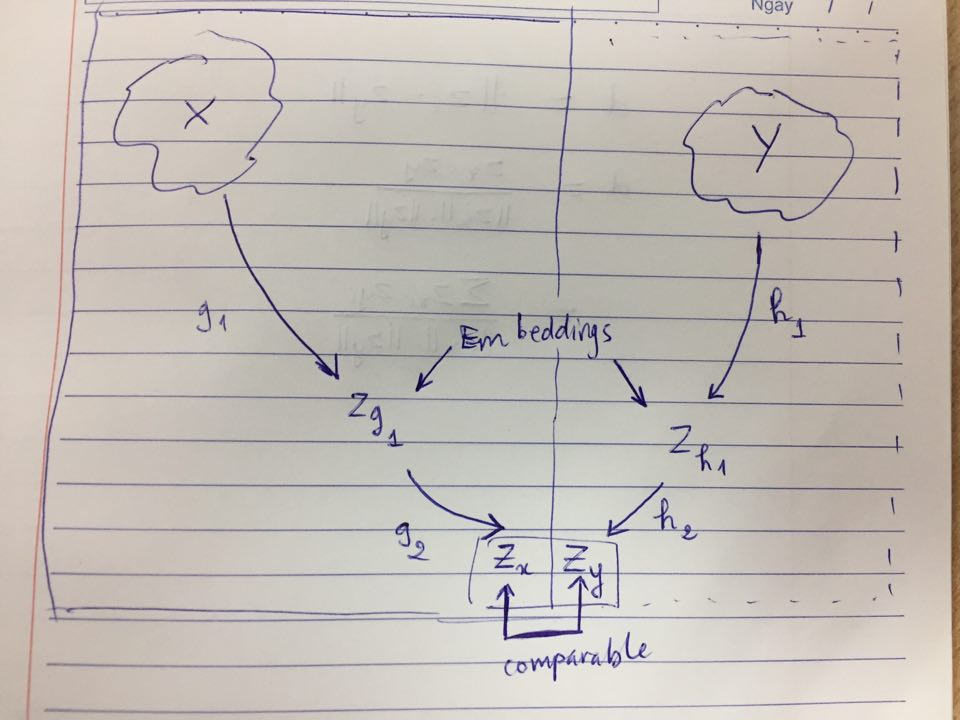
\includegraphics[width=10cm\textwidth]{Mohinh}
    \caption{Mô hình chung machine learning}
\end{figure}

Mô hình chung là tìm hàm $f: X \rightarrow Y$ với $X$ là bộ cơ sở dữ liệu và $Y$ là các đầu ra sao cho hàm $f$ với bộ dữ liệu $X$ thì cho đầu ra $Y$ hiệu quả nhất.\\
Một mô hình chung có thể biểu diễn như sau :
\begin{align*}
X \overset{h_1}{\rightarrow}  Z_{h_{1}} \overset{h_2}{\rightarrow} Z_X \textbf{(1)} \\  
Y \overset{g_1}{\rightarrow}  Z_{g_{1}} \overset{g_2}{\rightarrow} Z_Y \textbf{(2)}
\end{align*}
Với $h_1,g_1,h_2,g_2$ là các \textbf{basis function}.\\
Hàm $h_2,g_2$ dùng để đưa các $Z_{g_{1}},Z_{h_{1}}$ và tạo ra được tương ứng $Z_X,Z_Y$ vào không gian hàm chung. Từ đó đưa ra so sánh giữa $Z_X,Z_Y$.
Để so sánh ta dùng $$d(Z_X,Z_Y)=P(X,Y _{g_{1},g_{2},h_{1},h_{2}})$$\\
\newpage
Trong đó $P$ là hàm để đó \textbf{Performance Measure}\\
Có nhiều cách tính $d$ và $P$ ,chẳng hạn
\begin{align*}
    d(X_1,X_2)&=\sqrt {\sum (x_{ij_1}-x_{ij_2})^2 } \textbf{(3)}\\
    d(X_1,X_2)&=\dfrac{\sum {x_{ij_{1}} \cdot x_{ij_{2}}}}{||x_ij_{1}|| \cdot ||x_ij_{2}||} \textbf{(4)} \\
    d(X_1,X_2)&=-\sum p_{X_{1}i}log(p_{X_{2}i})
\end{align*}
\section{Linear Regression}
Ta sẽ lấy ví dụ theo mô hình trên. \\
Lấy $X$ là tập hợp các tính chất của một căn nhà ví dụ vị trí địa lý, kích thước, độ bền,....\\
$Y$ là tập hợp giá trị của căn nhà.\\
Việc sử dụng Linear Regression theo mô hình trên là việc mã hoá $Z_{g_{1}}$
Như mô tả ở mô hình chung, khi đưa $X$ qua basis function $h_1$ sẽ cho ta được các toạ độ (coordinates) $Z_{g}_{1}$. Từ các toạ độ, bước $h_2$ sẽ là từ $Z$ ta nhân vô hướng với một vector $w$ cột ví dụ như $$w=[r_1,r_2,...,r_N]^T$$ để dự đoán giá nhà $\widehat{y}$  và so sánh nó với giá trị thực (linear).Ở dạng công thức toán ta có thể viết là
$$\widehat{y}=Z^{T}w $$
Từ đây ta điều chỉnh $d(y,\widehat{y})$
(\textbf{Performance Measure}) sao cho sai số của đầu ra đạt giá trị nhỏ nhất. Hay nói cách khác là ta cần tìm $w^*$ sao cho
$$w^*=argmin \sum_{i=1}^{N}d(y,\widehat{y})$$
Với tập dữ liệu $D={\{(x_i,y_i)\}}_{i=1}^{N}$

\section{Classification}
Một số hàm toán sử dụng \\
Hàm \textbf{sigmoid} $$\sigma(x)=\dfrac{1}{1+e^{-x}}$$
Hàm \textbf{softmax} $$a_i=\dfrac{\sigma(x_i)}{\sum_{i=1}^{n}\sigma(x_i)}$$
Hàm \textbf{ReLU} 
\begin{align*}
    f(g(x))=
    \begin{cases}
        0 , &g(x)<0\\
        g(x) , &g(x) \ge 0
    \end{cases}
\end{align*}
\subsection{Linear Classification}
Đối với Linear Classification, ta có 2 thuật toán cơ bản của bài toán là Logistic Regression và Softmax Regression.\\ 
Bài toán Logistic Regression thường sử dụng để giải quyết các bài toán \textbf{binary classification}. Còn bài toán Softmax Regression thì sử dụng để giải quyết những bài toán có nhiều class hơn. \\
Theo mô hình chung trên, nguyên tắc hoạt động chung của hai hàm là ta được cung cấp dữ liệu là vector toạ độ $Z_{g_{1}}$ và ta cần đưa đầu ra là $Z_Y$. Để làm được như vậy trước hết ta đưa $Z_{g_{1}}$ qua một \textbf{basis function} $g_2$ (linear) và sau đó điều chỉnh $d(y,\widehat{y})$ để cho ra được một vector $\widehat{y}$ là các \textbf{probability vector}.\\
\textbf{Định nghĩa} : \textbf{probability vector} là vector $\widehat{y}=[p_{y_{1}},p_{y_{2}},...,p_{y_{n}}]^T$ (với Linear Classification) thoả các điều kiện sau 
\begin{itemize}
    \item $(0 \le p_i \le 1)_{i=1}^{n}$
    \item $\sum_{i=1}^{n}p_i=1$
\end{itemize}
Để so sánh $\widehat{y}$ và $y$ ta cũng cần chuyển vector $y$ về probability vector dùng \textbf{hot coding}. 
Hàm để tính $d(y,\widehat{y})$ (Performance Mesuare) là hàm \textbf{cross-entropy} với công thức $$d(y,\widehat{y})=-\sum_{i=1}^{n}y_ilog(\widehat{y_{i}}) $$

\subsection{Nonlinear Classification (Multi-layer Perceptron)}
Xét về mô hình chung thì Nonlinear và Linear cũng có nhiều điểm tương đồng như việc tính $d(y,\widehat{y})$ hay đầu ra $\widehat{y}$ đều là probability vector
Xét theo mô hình chung của machine learning ,điểm khác nhau giữa Nonlinear và Linear là ở bước $g_2$. Bước $g_2$ của Nonlinear sẽ được thông qua thêm nhiều bước ẩn (hidden layers). Biểu diễn của toán học là
\begin{align*}
    a&=\gamma(\dot{W_{z}}\dot{z})\\
    \widehat{y}&=(\dot{W_{a}}\dot{a})
\end{align*}
Trong đó hàm $\gamma(x)$ là một hàm phi tuyến (nonlinear)
\end{document}